\documentclass{article} % For LaTeX2e
\usepackage{nips15submit_e,times}
\usepackage[colorlinks,linkcolor=red]{hyperref}
\usepackage{url}
\usepackage{amsmath}
\usepackage{graphicx}
\usepackage{float}
\usepackage{bm}
\usepackage{amssymb}
%\documentstyle[nips14submit_09,times,art10]{article} % For LaTeX 2.09


\title{CS499 Homework 8 (First Draft)}


\author{
	Intersteller\thanks{ Use footnote for providing further information
		about author (webpage, alternative address)---\emph{not} for acknowledging
		funding agencies.}
	Department of Computer Science
	Cranberry-Lemon University
	Pittsburgh, PA 15213
}

% The \author macro works with any number of authors. There are two commands
% used to separate the names and addresses of multiple authors: \And and \AND.
%
% Using \And between authors leaves it to \LaTeX{} to determine where to break
% the lines. Using \AND forces a linebreak at that point. So, if \LaTeX{}
% puts 3 of 4 authors names on the first line, and the last on the second
% line, try using \AND instead of \And before the third author name.

\newcommand{\fix}{\marginpar{FIX}}
\newcommand{\new}{\marginpar{NEW}}

%\nipsfinalcopy % Uncomment for camera-ready version

\begin{document}

	\maketitle
	\textbf{Exercise 8.1}\par
	\quad 1.\par
  	\begin{figure}[H]
  	\centering
  	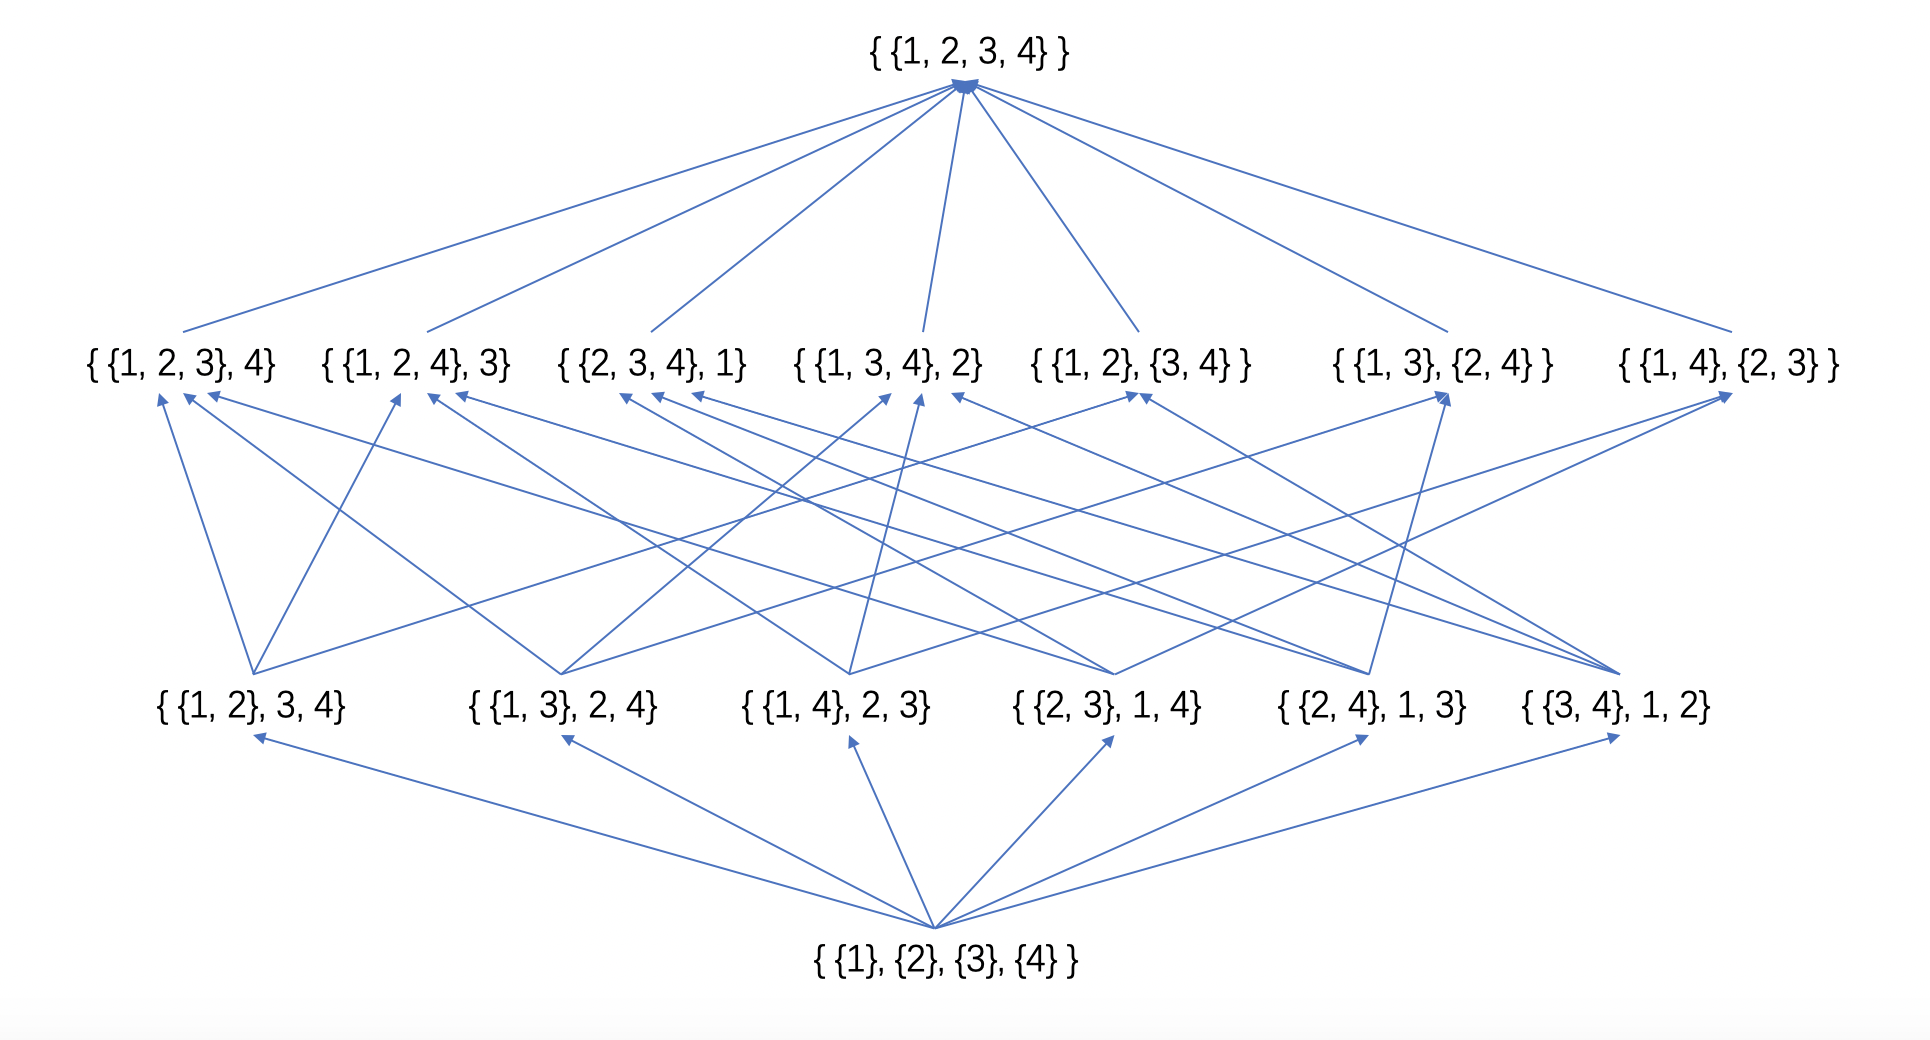
\includegraphics[scale=0.5]{8_1.png}
  	\caption{}
  	\label{}
  	\end{figure}
	\quad 2. The size of the largest chain is $4$.\par
	 \quad 3. The size of the largest antichain is $7$.\par
	
	\textbf{Exercise 8.2}\par
    $1.(1,1,1,1,1,\cdots)$ are minimal. There is not a maximum.\par
    $2.$There is a minimum, but there is not a maximum.\par
    $3.$Yes. For example,\par
    $$(1,1,1,1,\cdots)$$
    $$(2,1,1,1,\cdots)$$
    $$(3,1,1,1,\cdots)$$
    $$(4,1,1,1,\cdots)$$
    $$\vdots$$
    $4.$Yes.For example.\par
    $$(1,2,3,\cdots,k)$$
    $$(2,1,3,\cdots,k)$$
    $$(2,3,1,\cdots,k)$$
    $$\vdots$$
    $$(2,3,4,\cdots,k,1)$$

	\textbf{Exercise 8.3}\par
    Yes. We prove it by mathematical induction.\par
    $(1)$When $n=1$, obviously, we can sort elements from small to large to get an infinite chain.\par
    $(2)$We suppose every infinite subset $S \subseteq N_0^N$ contain an infinite chain, then when $n=N+1$, we can take the first element of each set to constitute a sequence and sort the sequence from small to large. There are two situations:\par
    $1.$The sequence is bounded.\par
    Obviously at least one element we call it $a$ has appeared countless times. Based on the inductive assumption, we can find an infinite chain in all sets whose first element is $a$ and whose $a$ is removed. Then we add $a$ back to these sets which constitute the infinite chain to get the final infinite chain.\par
    $2.$The sequence is unbounded.\par
    We take the set $A$ whose first element is smallest in this sequence as the first set in the chain. Based on the inductive assumption, we can find an infinite chain contained this set which remove the first element in all sets removing their first elements. Obviously the successor of the set $A$ removing its first element in this chain will be the successor of $A$ in the final chain if it adds its first element and we call it $B$. In the sorted sequence, there are infinite elements after the first element of $B$ and we can find an infinite chain in the sets contained these elements as their first elements and removing their first elements. So we can find the successor of $B$ in the final chain. And so on, we get an infinite chain when $n=N+1$.\par
    So every infinite subset $S \subseteq N_0^n$ contain an infinite chain.


	\textbf{Exercise 8.4}\par
	We assume that $(\mathbb{N}_{0}^{n},\leq)$ has an infinite antichain $T$. Obviously, $T \subseteq  (\mathbb{N}_{0}^{n},\leq)$.
	According to \textbf{exercise 8.3}, we get $T$ contains an infinite chain, which contradicts $T$ is an infinite antichain.
	Thus $(\mathbb{N}_{0}^{n},\leq)$ has no infinite antichain.\par
	\textbf{Exercise 8.5}\par
	$n=2$\par
	 \begin{figure}[H]
  	\centering
  	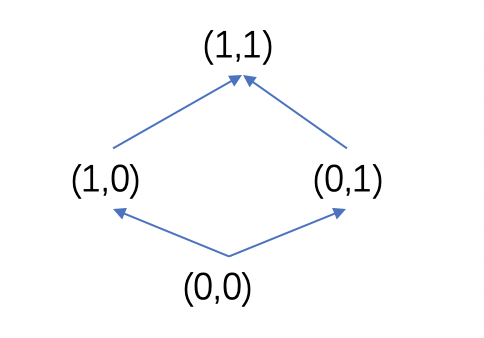
\includegraphics[scale=0.5]{8_5_1.png}
  	\caption{}
  	\label{}
  	\end{figure}
	$n=3$\par
	\begin{figure}[H]
  	\centering
  	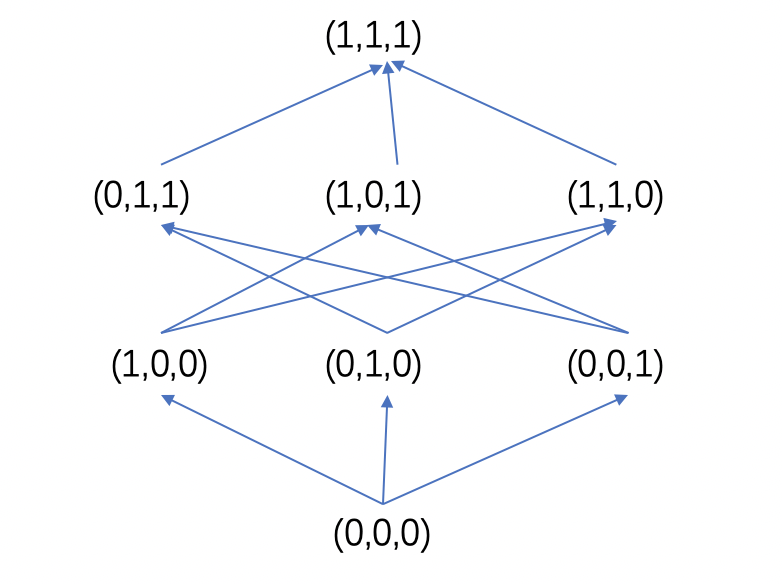
\includegraphics[scale=0.5]{8_5_2.png}
  	\caption{}
  	\label{}
  	\end{figure}
	\textbf{Exercise 8.6}\par
	Maximum is $(\underbrace{1,1,1,\cdots,1}_{n})$\par
	Minimum is $(\underbrace{0,0,0,\cdots,0}_{n})$\par
	Maximal is  $(\underbrace{1,1,1,\cdots,1}_{n})$\par
	Minimal is $(\underbrace{0,0,0,\cdots,0}_{n})$\par
	\textbf{Exercise 8.7}\par
	We construct the Hasse diagrams like \textbf{Exercise 8.5}.
	The first layer is an element with $n$ one. The second layer is $n$ elements with $n-1$ one.
	The third layer is $\binom{2}{n}$ elements with $n-2$ one......The $k$ layer is $\binom{k-1}{n}$ elements with $n+1-k$ one, where $1\leq k\leq n+1$.\par
	Obviously elements in the same layer is antichain, since elements in chain must have different numbers of one and in the same layer the number of one is equivalent.
	Thus it has $n+1$ antichain partition.\par
	According to Mirsky's Theorem, max size of chain$=$min size of antichain partition. It means max size of chain must less than or equal to the size of each antichain partition.
	Thus the longest chain of ${\{0,1\}}^n$ $\leq n+1$. Since we get $n+1$ antichain partition in above Hasse diagrams, then the longest chain of ${\{0,1\}}^n$ is $n+1$.\par
	

	

	\textbf{Exercise 8.8}\par
	 The largest antichain of $\{0,1\}^n$ is $(_{[n/2]}^n)$.According to the Dilworth Theorem,the largest antichain equals to the minimum size of chain partition.\par
	 We define a layer as a set of strings containing same number of $'1'$ and is sorted by how many  $'1'$ a string in this layer contains.\par
	 \textbf{1.}There are $(_{[n/2]}^n)$ strings in the middle layer, which has the most strings. Since any two strings from the same layer are not comparable, there are at least $(_{[n/2]}^n)$ chain partitions.\par
	 \textbf{2.} All strings in any layer except the middle one can form chains with unique strings in its adjacent layer with the following method:\par
	 Assuming there are more $'1'$ than $'0'$ in this layer, we calculate a strings score by the following rules: scan the string from the beginning and the initial score is $0$, add one if current digit is $1$,minus one otherwise. Find the digit where the first highest score appears (which must be a $'1'$),change it to $0$. Then we get a string belongs to its adjacent layer and these two strings can form a chain(they are comparable).Now we prove that this string is unique:\par
	 Assume that there are two different strings that transform into a same string. Assume that the first string changes the i-th digit, and the other changes the j-th digit (with no loss of generality, assume $i<j$).  Then the i-th digit of the second string and the j-th digit of the first string are $0$, whereas other digits are the same. Assume that the score of the $(i-1)$-th digit is k.Then the score of the i-th digit is $k+1$ for the first string and $(k-1)$ for the second. Assume that the score of the $(j-1)$-th digit for the first string is $k+1+p$,then the score of the $(j-1)$-th digit for the second string is $k-1+p$.The score of the j-th digit for the second string is $k+p$. Since the changing digit is where the first largest score occurs, we have
	 $$
	 k+1 \ge k+1+p
	 $$
	 $$
	 k<k+p
	 $$
	 where we get $p\geq 0$ and $p>0$ which contradict each other. So  different strings cannot transform into a same string by the method. Similarly, if there are more $'0'$ than $'1'$ in the layer,we can use a similar method to form chains with unique strings in its adjacent layer.
	
	\textbf{Question:}\par
	\textbf{1}How to prove the proposition that the set of integer has the smallest cardinality among all the infinite sets?
	\textbf{1}How to handle the Russell's paradox?
	


\end{document}
	

